\section{Trochoidal motion model}

\begin{figure*}
  \centering
  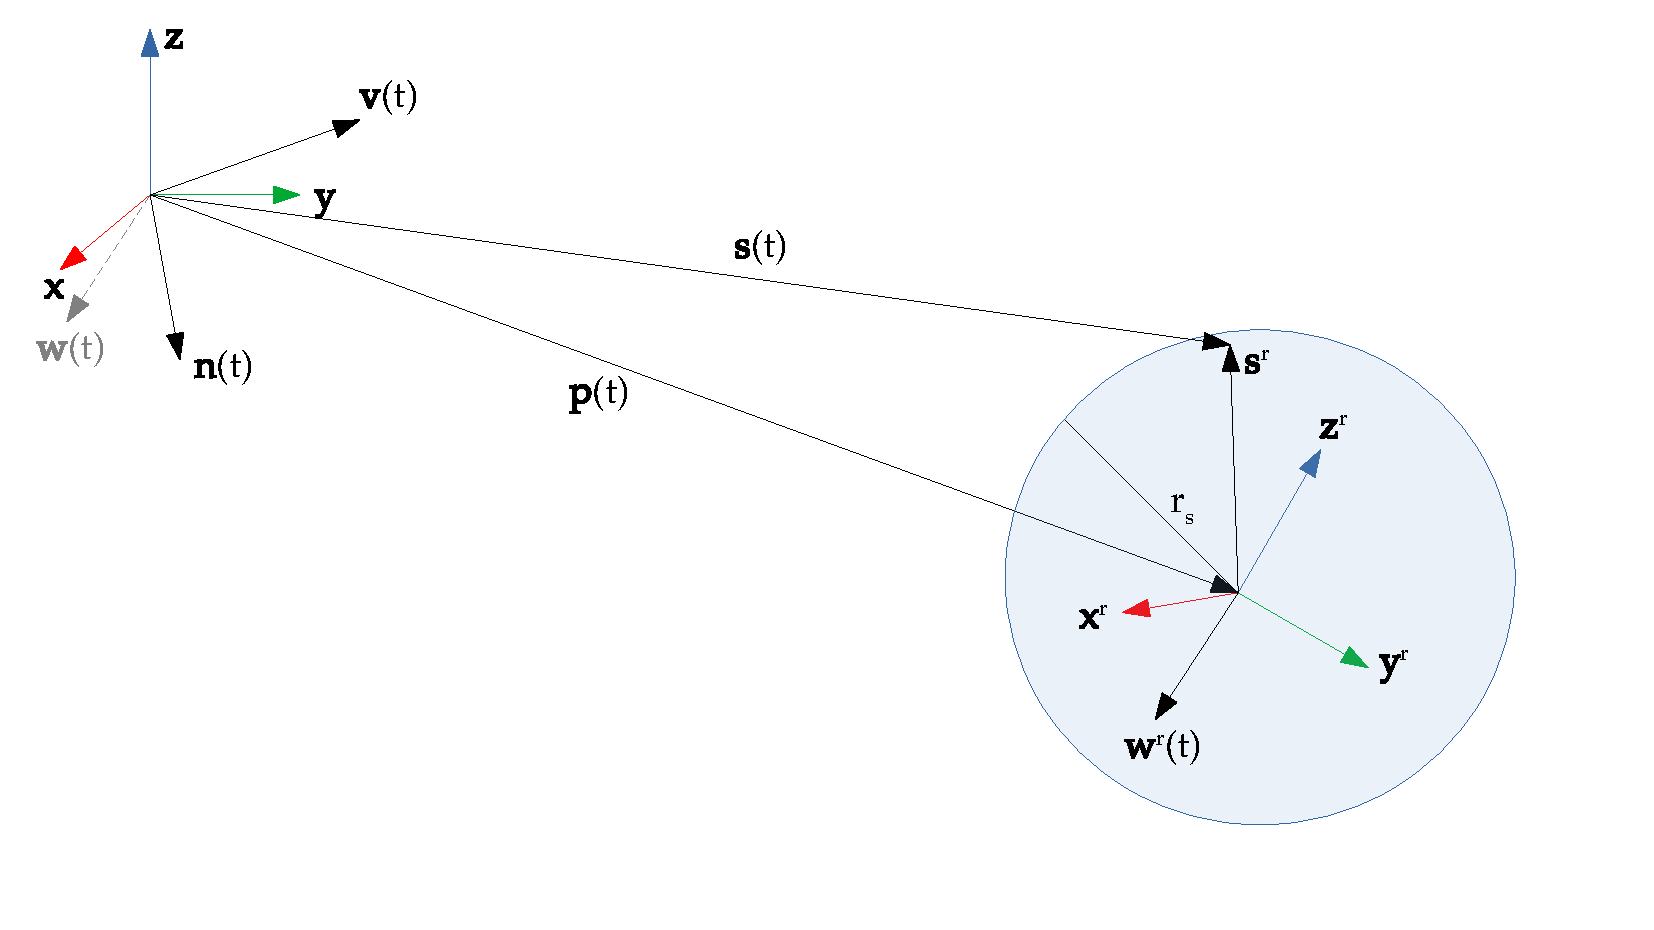
\includegraphics[width=.8\textwidth]{img/schematics}
  \caption{Schematics of the motion model}
  \label{fig:schematics}
\end{figure*}

The sensors rotation around the balls center is described through the rotation derivative which correspond to local gyro measurements $\vec{\omega}^r$   
\begin{align}
\frac{d}{dt}{\mathbf{R}}_r = \vec{\omega}^r_{\times} \cdot \mathbf{R}_r \;\; ,
\end{align}
where the cross-product matrix is defined as 
\begin{align}
\vec{\omega}_{\times} = 
\begin{pmatrix}
0 & -\omega_3 & \omega_2\\
\omega_3 & 0 & -\omega_1\\
-\omega_2 & \omega_1 & 0
\end{pmatrix} \;\; .
\end{align}
Go study group theory and learn about the Lie algebra $\mathfrak{so}(3)$ which is the tangent space to $\textrm{SO}(3)$ at its identity, to find out why this works. 
Anyways, through the inverse rotation we transform the local measurements into the global frame, leading to 
\begin{align}
\vec{\omega} = \mathbf{R}_r^{-1} \cdot \vec{\omega}^r
\end{align}
and
\begin{align}
\vec{s} = \mathbf{R}_r^{-1} \cdot \vec{s}^{\,r} + \,\vec{p}
\end{align}
with 
\begin{align}
\vec{p}(t) = \int_0^t \vec{v}(\tau) d\tau \;\; ,
\end{align}
where the velocity of the balls center over ground with normal $\vec{n}$ is
\begin{align}
\vec{v} = r_s \vec{\omega} \times \vec{n}\;\; .
\end{align}
The combined model:
\begin{align}
\vec{s} = \mathbf{R}_r^{-1} \cdot \vec{s}^{\,r} + \int \left( \left[ \mathbf{R}_r^{-1} \cdot r_s \cdot \vec{\omega}^r \right] \times \vec{n}\right)
\end{align}
expands, not ommiting the time dependence, to:
\begin{small}
  \begin{align}
    \vec{s}(t) &= \left[ \int_0^t \vec{\omega}^r_{\times}(\tau)\mathbf{R}_r(\tau)d\tau \right]^{-1} \vec{s}^{\,r} \\ \nonumber
    &+ \int_0^t\left( \left[ \bigg\{ \int_0^t \vec{\omega}^r_{\times}(\tau)\mathbf{R}_r(\tau)d\tau \bigg\} ^{-1} r_s \vec{\omega}^r(\tau) \right]\times \vec{n}(\tau) \right) d\tau
  \end{align}
\end{small}
which is the kinematic model to be solved numerically for any arbitrary gyro measurements.

% \section{Extended Kalman filter}